%%%%%%%%%%%中文essay模板 by whzecomjm in SUSTC%%%%%%%%%%%%%%%%%%%%%%%%%
\documentclass[a4paper,12pt]{article}
\usepackage{CTeX,graphicx}
\usepackage{amsmath}                  %%%加入vmatix,pmatrix,equation

%%%%%%%%%%%%%%%%%更改页面布局%%%%%%%%%%%%%%%5
\usepackage{fancyhdr}
\addtolength{\voffset}{-2.0cm}
\addtolength{\hoffset}{-1.0cm}
\addtolength{\textwidth}{2cm}
\addtolength{\headheight}{1.5cm}
\addtolength{\marginparwidth}{-2.5cm}

%%%%%%%%%%%%页眉的logo,use pdftexify%%%%%%%%%%
\pagestyle{fancy}
\newbox\schoolbadge
\setbox\schoolbadge=\hbox{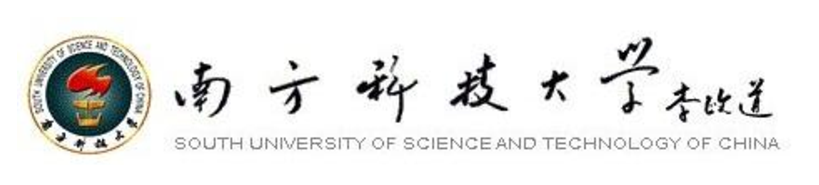
\includegraphics[width=0.5\textwidth]{logo}}
\lhead{\strut{\lower5pt\copy\schoolbadge}\strut}





%%%CTeX章节标题设置%%%%%%%%%%%%%%%
%\CTEXsetup[name={第,节}]{section}
%\CTEXsetup[name={第,小节}]{subsection}%中文名字
%\CTEXsetup[number={\chinese{section}}]{section}%中文数字



%%%theorem环境%%%%%%%%%%%%%%%%%%%%%%
\usepackage{amsthm}
\newtheorem{thm}{定理~}
\newtheorem{lem}{引理~}
\newtheorem{prop}{命题~}
\newtheorem{cor}{推论~}
\newtheorem{defn}{定义~}
\newtheorem{conj}{猜想~}
\newtheorem{exmp}{例~}
\newtheorem{rem}{注~}




%%%%证明环境%%%%%%%%%%%%
%\makeatletter
%\renewenvironment{proof}[1][\proofname]{\par
%    \pushQED{\qed}%
%    \normalfont \topsep6\p@\@plus6\p@ \labelsep1em\relax
%    \trivlist
%    \item[\hskip\labelsep\indent
%        \bfseries #1]\ignorespaces
%}{%
%    \popQED\endtrivlist\@endpefalse
%}
%\makeatother
%\renewcommand{\proofname}{证明}




%%%%%%%%%%%%%%%%%%%%%%%%%%%%%%%%%%%%%%%%%%%%%%%%%%%%%%%%%%%%%%%%%%
\begin{document}
\numberwithin{equation}{subsection}    %%公式编号按小节


%%%%%%%%%%%%%%%%%%%%%%%%%%%标题页内容%%%%%%%%%%%%%

\title{常微分方程的数值解法}
\vspace{10cm}
\date{\today}
\author{张文超\ 王嘉乐\ 骆韬}
\maketitle
\renewcommand{\contentsname}{目录}
\tableofcontents
\newpage


%%%%%%%%%%%%%%%%%%%%%%%%%%摘要与关键词%%%%%%%%%%%%%%%%%%%%

\begin{flushleft}
\textbf{摘要}:本文总结了多种常微分方程的数值解法,并且给出了相应的\textbf{Matlab}的实现方式。我们比较了这几种经典的算法的误差大小。
同时,我们还给出了自己的一个新的变步长的算法,它的精确度能够达到一个比较高的水平,在评估该算法时,我们用到了一种新的评估方式。
\end{flushleft}

\begin{flushleft}
\textbf{关键词}:常微分方程;数值解法;欧拉法;辛普森法;泰勒级数法;变步长
\end{flushleft}


%%%%%%%%%%%%%%%%%%%%%%正文%%%%%%%%%%%%%%%%%%%%%%%%
\section{问题的简述}
一阶常微分方程的初值问题用如下形式描述:
\begin{equation}
    \left\{
      \begin{array}{ll}
        y'(x)=f(x,y) & a\leq x\leq b \\
        y(x_0)=y_0
      \end{array}
    \right.
\end{equation}
\begin{flushleft}
    其中,$y_0$是已知常数。
\end{flushleft}
对于上式,只要$f(x,y)$适当的光滑,比如满足关于$y$的李普希兹条件\cite{lip}:
\[\|f(x,y)-f(x,\overline{y})\|\leq L\|y-\overline{y}\|\footnote{${\bar y_{k + 1}} = y\left( {{x_k}} \right) + f \left( {{x_k},y\left( {{x_k}} \right)} \right)$}\]
其中$L$为常数,理论上就可以保证式$(1.0.1)$的解$y=y(x)$存在并且唯一。但是,实际计算中
只有少数的特殊的微分方程可以用解析方法来求解,绝大多数的一阶常微分方程都难以求得其精
确解。为此,数值方法提供了实际应用一种有效的途径。

\section{数值方法的基本思想}
常微分方程初值问题的解$y(x)$在$[a,b]$上的有限个值$y(x_k)$的近似值$y_k$称为常微分方程的初值问题的数值解,
其中$x_k=x_{k-1}+h_{k-1},k=1,2,3\ldots,n$。其中$x_k$称为节点,$h_k$为步长。数值方法的基本思想是根据已知的或已求出的节点上的
函数值计算当前节点上的函数值,一步一步向前推进。因此只需建立由已知的或已求出的节点上的函数值求当前节点函数值的递推公式即可。\par
数值方法的一般步骤是:
\begin{itemize}
\item [第一步] 用节点$a=x_0,x_1,\cdots,x_n=b$将区间$[a,b]$分成$n$份,节点$x_0,x_1,\cdots,x_n=b$满足$a=x_0<x_1<\ldots<x_n=b$。
\item [第二步] 用数值方法求出函数$y(x)$在节点$x_k$处的函数值$y(x_k)$的近似值$y_k,k=1,2,\ldots,n$。
\item [第三步] 根据已得到的列表函数$(x_k,y_k)$,$k=0,1,\ldots,n$,给出$y(x)$的近似。
\end{itemize}

很容易看出第二步是关键,即如何根据方程$y'(x)=f(x,y)$及初始条件$y(x_0)=y_0$。给出$y(x)$在各节
点的近似值$y(x_k)$,换句话讲,如何根据$y'(x)=f(x,y)$及初始条件$y(x_0)=y_0$实现从$y(x_k)$到$y(x_{k+1})$的过渡,这是微分方程
数值解法的关键。所以不同的方法其不同之处就是取决于这个过渡的不同。从$y(x_k)$到$y(x_{k+1})$过渡的几种常用途径,并按照这些途
径就能给出解微分方程初值问题的几种常见方法。

\section{基本的几个数值方法}
\subsection{欧拉法}
\subsubsection{欧拉法原理}
\begin{defn}[欧拉方法]
    将区间$[a,b]$ $n$等分,步长为 $h=(b-a)/n$ ,得到$n+1$个分点。已知$y(x_0)=y_0$,取区间$[x_k,x_{k+1}]$对方程$(1.0.1)$两端积分,得到
\begin{eqnarray*}
    \int_{{x_k}}^{{x_{k + 1}}} {y'(x)dx}  &=& \int_{{x_k}}^{{x_{k + 1}}} {f(x,y(x))dx} \\
    \text{即}y({x_{k + 1}}) - y({x_k}) &=& \int_{{x_k}}^{{x_{k + 1}}} {f(x,y(x))dx}
\end{eqnarray*}
右边的积分用左矩形公式代替,则有
\begin{equation}
    y({x_{k + 1}}) - y({x_k}) \approx hf({x_k},y({x_k}))
\end{equation}
这个近似值我们表示为:
\begin{equation}
    {y_{k + 1}} = {y_k} + hf({x_k},{y_k})
\end{equation}
于是我们得到求解问题的欧拉法:
\begin{equation}
\left\{ \begin{array}{l}
{y_{k + 1}} = {y_k} + hf({x_k},{y_k}),\quad i = 1,2, \cdots ,n - 1\\
{y_0} = y({x_0})
\end{array} \right.
\end{equation}
\end{defn}

\subsubsection{欧拉法的收敛性}
\begin{defn}[数值方法的收敛性]
    数值方法的收敛性是指给出的数值解$y_n$当$h\rightarrow0$时是否收敛到微分方程的解$y(x_n)$,即是否成立$y_n \rightarrow y(x_n)$,$h\rightarrow0$。
\end{defn}

关于欧拉法的收敛性\cite{converge}的证明很多教材会有提到,我们主要是利用这个定义,在接下来我们的变步长的方法中证明其收敛性。

\subsection{R-欧拉法(Righthand)}
将欧拉法的式$(3.1.1)$换成右矩形对应的式子,即:
\begin{equation}
    y({x_{k + 1}}) - y({x_k}) \approx hf({x_{k+1}},y({x_{k+1}}))
\end{equation}
从而有:
\begin{equation}
    {y_{k + 1}} = {y_k} + hf({x_{k+1}},{y_{k+1}})
\end{equation}
则欧拉法就会变成相应的R-欧拉法。值得注意的是,R-欧拉法不是显式的,即等号右边的$y_{k+1}$是用欧拉法预估的值。相当于是欧拉法的
一种反馈算法。

\subsection{梯形法}
梯形法实际上是欧拉法和R-欧拉法的平均值,因此在某种程度上有比欧拉法更高阶的精度。梯形法的表达式如下:
\begin{equation}
\left\{ \begin{array}{l}
{{\bar y}_{k + 1}} = {y_k} + hf({x_k},{y_k})\\
{y_{k + 1}} = {y_k} + \frac{h}{2}[f({x_k},{y_k}) + f({x_{k + 1}},{{\bar y}_{k + 1}})]
\end{array} \right.\quad
\end{equation}
或者写成一个表达式:
\begin{equation}
{y_{k + 1}} = {y_k} + \frac{h}{2}\left[ {f({x_k},{y_k}) + f\left( {{x_{k + 1}},{y_k} + h\,f({x_k},{y_k})} \right)} \right]
\end{equation}

\subsection{辛普森法}
欧拉法,R-欧拉法,梯形法都可以用Picard的方法推出,分别是用左矩形、右矩形、梯形来近似近似积分。辛普森法也是一种重要的近似方法,
它不再仅限于多边形的近似,而是用到了二次函数\footnote{更多参见大一微积分课本:Calculus Rigor:Concision,Clarity.Simpson's Rule.p189}。辛普森法对应的迭代公式为:
\begin{equation}
    y_{k+1}=y_{k-1}+\frac{h}{3}(f(x_{k+1},y_{k+1})+4f(x_{k},y_{k})+f(x_{k-1},y_{k-1}))
\end{equation}
和R-欧拉法一样,这里等号右边的$y_{k+1}$是用欧拉法预估的。值得注意的是,这种方法和前面三种方法不同,计算$y_{k+1}$还需要$y_{k-1}$
的值,因此,当我们计算$y_{2}$时,还要用欧拉法预估$y_0$。

\subsection{几种方法的比较表}
\begin{center}
\begin{tabular}{|l|l|l|l|}
\hline
 & 公式 & 局部截断误差 & 精度 \\
\hline
欧拉法 & ${y_{k + 1}} = {y_k} + hf({x_k},{y_k})$ & $\frac{{{h^2}}}{2}{y^{(2)}}\left( {{x_n}} \right)$ & 1阶 \\
R-欧拉法 & ${y_{k + 1}} = {y_k} + hf({x_{k+1}},{y_{k+1}})$ & $-\frac{{{h^2}}}{2}{y^{(2)}}\left( {{x_n}} \right)$ & 1阶 \\
梯形法 & ${y_{k + 1}} = {y_k} + \frac{h}{2}f({x_k},{y_k}) + f\left( {{x_{k + 1}},{y_k} + h\,f({x_k},{y_k})} \right) $ & $\frac{{{h^3}}}{3}{y^{(3)}}\left( {{x_n}} \right)$ & 2阶   \\
辛普森法 & $y_{k+1}=y_{k-1}+\frac{h}{3}(f(x_{k+1},y_{k+1})+4f(x_{k},y_{k})+f(x_{k-1},y_{k-1}))$ & $ - \frac{{{h^4}}}{{180}}{y^{(4)}}\left( {{x_n}} \right)$ & 3阶  \\
\hline
\end{tabular}
\end{center}
\subsection{泰勒级数法}
泰勒级数法的出发点和辛普森法是一样的,都是用曲线下方的面积去近似积分。不过它们做出来的方式又是不一样的,辛普森法是一种用三个点
决定一条抛物线,然后用抛物线下方的面积来近似。而泰勒级数法所得到的曲线\footnote{比如当泰勒级数取二阶时,也是一个抛物线(或者是
退化曲线)}是基于一个点,但是需要这个点更多的信息,即更高阶的导数。\par
对于方程$(1.0.1)$,假设其解为$y=y(x)$,则将$y(x_{k+1})$展成$y(x_{k})$的泰勒级数如下:
\begin{equation}
y\left( {{x_{k + 1}}} \right) = y\left( {{x_k}} \right) + hy'\left( {{x_k}} \right) + \frac{{{h^2}}}{2}y''\left( {{x_k}} \right) + \frac{{{h^3}}}{6}y'''\left( {{x_k}} \right) + \cdots
\end{equation}
具体的导数求法如下:
\begin{equation}
\begin{array}{l}
y' = f(x,y) \equiv {f^{(0)}}\\
y'' = \frac{{\partial f}}{{\partial x}} + \frac{{\partial f}}{{\partial y}}\frac{{dy}}{{dx}} = \frac{{\partial {f^{(0)}}}}{{\partial x}} + \frac{{\partial {f^{(0)}}}}{{\partial y}}f \equiv {f^{(1)}}\\
y''' = \frac{{\partial {f^{(1)}}}}{{\partial x}} + \frac{{\partial {f^{(1)}}}}{{\partial y}}f \equiv {f^{(2)}}\\
 \cdots \\
{y^{(j)}} = \frac{{\partial {f^{(j - 2)}}}}{{\partial x}} + \frac{{\partial {f^{(j - 2)}}}}{{\partial y}}f \equiv {f^{(j - 1)}}\\
 \cdots
\end{array}
\end{equation}

要使公式具有p阶精度,则在$(3.5.1)$式中截取前$p+1$项,用$(3.5.2)$式计算各阶导数,即得下面Taylor公式:
\begin{equation}
{y_{k + 1}} = {y_k} + h{y'_k} + \frac{{{h^2}}}{2}{y''_k} +  \cdots  + \frac{{{h^p}}}{{p!}}y_k^{(p)}
\end{equation}
局部的截断误差为:
\[ y\left( {{x_{n + 1}}} \right) - {y_{n + 1}} \approx \frac{{{h^{p + 1}}}}{{\left( {p + 1} \right)!}}{y^{(p + 1)}}\left( \xi  \right){\rm{,    }}{x_n} < \xi  < {x_{n + 1}}\]

\section{基本数值方法的Matlab实现}
基本的思想和迭代的公式上文已经提及,所以这几种固定步长的Matlab实现,主要体现Matlab的运用技巧。
\subsection{基本的欧拉法Matlab代码}
欧拉法的Matlab代码\footnote{此代码由骆韬提供}比较简单,但却相当于是所有等步长的代码的模板。下面给出了欧拉法的代码:
\begin{quote}
\small{
syms x y\\
f = x$\wedge$2 - y; \% dy/dx = f\\
x0 = -2.5 ; y0 = 1 ; \% 初值\\
h = 0.3; \% 步长\\
n = 10; \% 步数\\
c = [x0,y0];\\
for i = 2:n\\
    c(i,1) = c(i-1,1) + h;\%xi的迭代\\
    c(i,2) = c(i-1,2) + subs(f,[x,y],[c(i-1,1),c(i-1,2)])*h;\%yi的迭代\\
end\\
plot(c(:,1),c(:,2))\%作图
}
\end{quote}
对于其他的数值方法需要相应改变的地方主要就是第9行和第10行,欧拉法的结果图如Figure 1。
\begin{figure}
\centering
  % Requires \usepackage{graphicx}
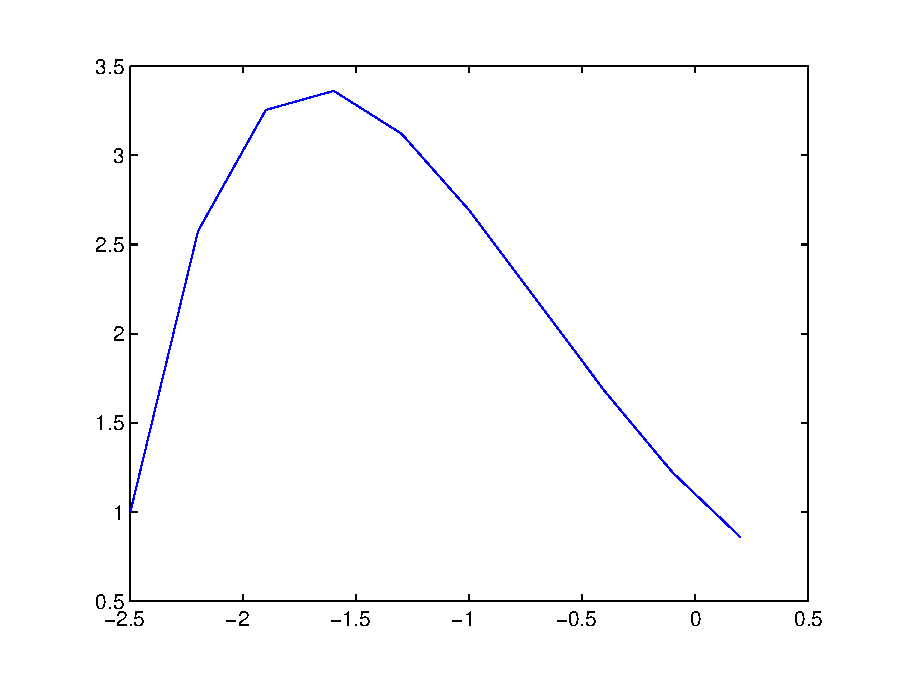
\includegraphics[width=0.65\textwidth]{Euler}
\caption{欧拉法}
\end{figure}



\subsection{欧拉法、R-欧拉法、梯形法和辛普森法的Matlab实例误差对比}
我们先通过一个实例来评估一下这几种方法的“优劣性”,之所以将Taylor方法和其它的方法分开,是因为欧拉法存在多一个预设参数——阶数$n$,
因此很难直接有比较的平台。并且前文也提到了这四种方法的实质就是用其他图形来代替积分曲线下方的面积。因而这些方法更有可比性。\par
我们通过求解如下初值问题来描述这几种方法的相对“优劣性”:
\begin{equation}
    \left\{
      \begin{array}{ll}
        y'(x)=2y \\
        y(0)=1
      \end{array}
    \right.
\end{equation}

以下是比较的代码\footnote{此代码由王嘉乐提供}的局部\footnote{省去了一些值的定义,这些可以参见欧拉法代码},我们用到的步长
是$0.1$,步数为$50$步:
\begin{quote}
\small{
    k1 = subs(f,[x,y],[w,q]);\\
    k2 = subs(f,[x,y],[c(i-1,1),c(i-1,2)]);\\
    k3 = subs(f,[x,y],[c(i,1),k]);\\
    c(i,2) = q + h*(k1+4*k2+k3)/3;\\
    else\\
    kk = c(i-1,2) + subs(f,[x,y],[c(i-1,1),c(i-1,2)])*h;\\
    c(i,1) = c(i-1,1) + h;\\
    kk1 = subs(f,[x,y],[c(i-2,1),c(i-2,2)]);\\
    kk2 = subs(f,[x,y],[c(i-1,1),c(i-1,2)]);\\
    kk3 = subs(f,[x,y],[c(i,1),kk]);\\
    c(i,2) = c(i-2,2) + h*(kk1+4*kk2+kk3)/3;\\
}
\end{quote}
\par
我们可以看到运行过后的图如下Figure 2\&3:
\begin{figure*}[thispage]
\begin{minipage}[t]{0.5\textwidth}
\centering
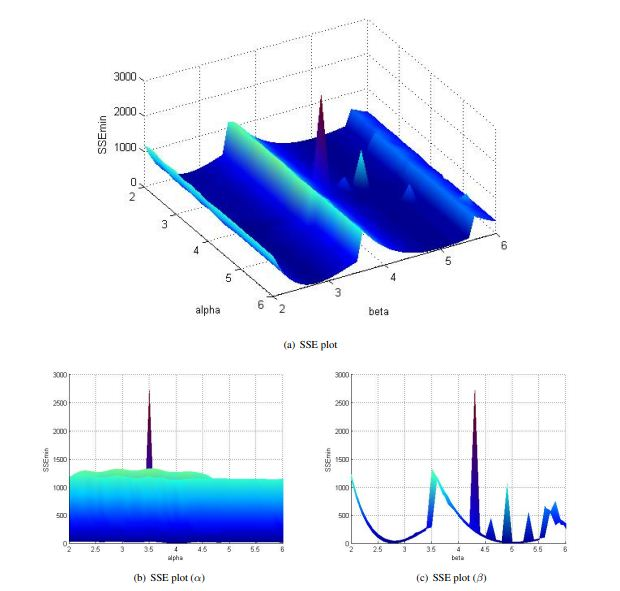
\includegraphics[width=\textwidth]{whole}
\caption{几种方法的比较}
\end{minipage}%
\begin{minipage}[t]{0.5\textwidth}
\centering
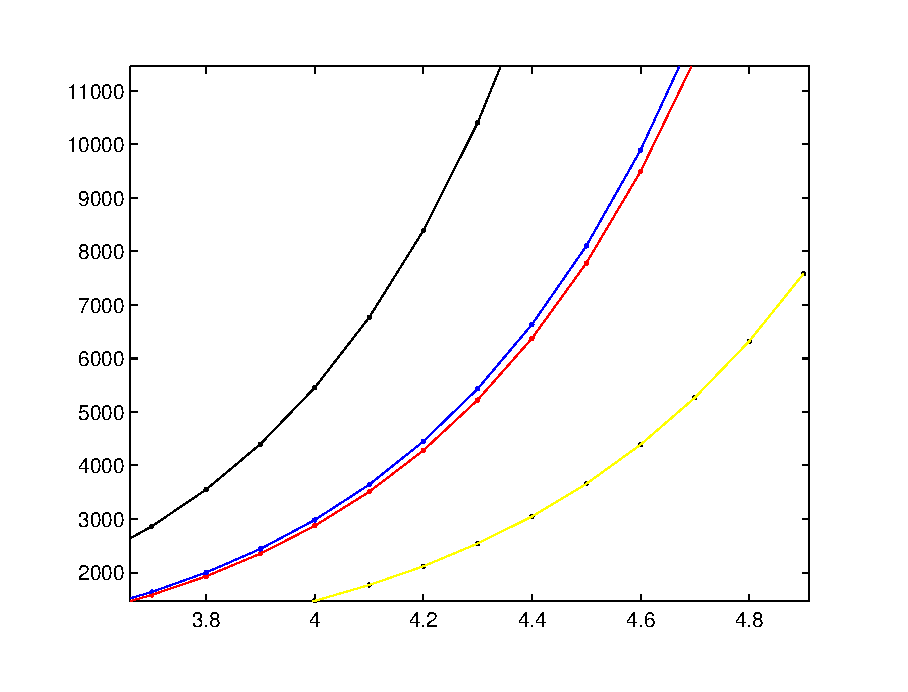
\includegraphics[width=\textwidth]{compare}
\caption{几种方法的比较放大图}
\end{minipage}%
\end{figure*}

\begin{center}
\begin{tabular}{|l|l|l|l|}
  \hline
点的横坐标&righthand&euler&simposons\\
  \hline
0.1&0.018597242&0.021402758&0.021402758\\
0.2&0.045775302&0.051824698&0.009158031\\
0.3&0.0845052&0.0941188&0.028127689\\
0.4&0.138672832&0.151940928&0.022112899\\
0.5&0.213343234&0.229961828&0.04083626\\
0.6&0.315098155&0.334132923&0.041612561\\
0.7&0.452466729&0.472019167&0.062709848\\
0.8&0.636474279&0.653215464&0.071897864\\
0.9&0.881340847&0.889867112&0.09886469\\
1&1.205369408&1.197319677&0.119574539\\
1.1&1.632074129&1.594929793&0.157424932\\
1.2&2.191612278&2.107075932&0.194965347\\
1.3&2.922599902&2.764417497&0.251197072\\
1.4&3.874412271&3.605462126&0.314207468\\
1.5&5.110096289&4.678515349&0.40027427\\
1.6&6.710054985&6.044104308&0.502503887\\
1.7&8.776705579&7.77798898&0.63607743\\
1.8&11.44036453&9.974901163&0.799158539\\
1.9&14.86667824&12.75318456&1.007614055\\
2&19.26599975&16.26055011&1.26536465\\
  \hline
\end{tabular}
\end{center}



\subsection{泰勒级数法的Matlab代码}
泰勒级数的算法\footnote{此代码由骆韬提供}除了有$y_k$的迭代,还有$n$阶导数的迭代。以下是泰勒法的Matlab代码局部:
\begin{quote}
\small{
for i = 2:n\\
c(i) = diff(c(i-1),x) + diff(c(i-1),y)*c(1); \% 各阶导数\\
subsc = subs(c,[x,y],[x0,y0]);\\
taylor = y0 ;\\
for i= 1:n\\
   taylor = taylor + (subsc(i)*(x-x0)$\wedge$i)/factorial(i);  \%n阶taylor展开\\
for i = 2:11\\
    b(i) = subs(taylor,[x0,y0,x],[a(i-1),b(i-1),a(i)]);\\
plot(a,b)\\
}
\end{quote}
\begin{figure}[thispage]
\centering
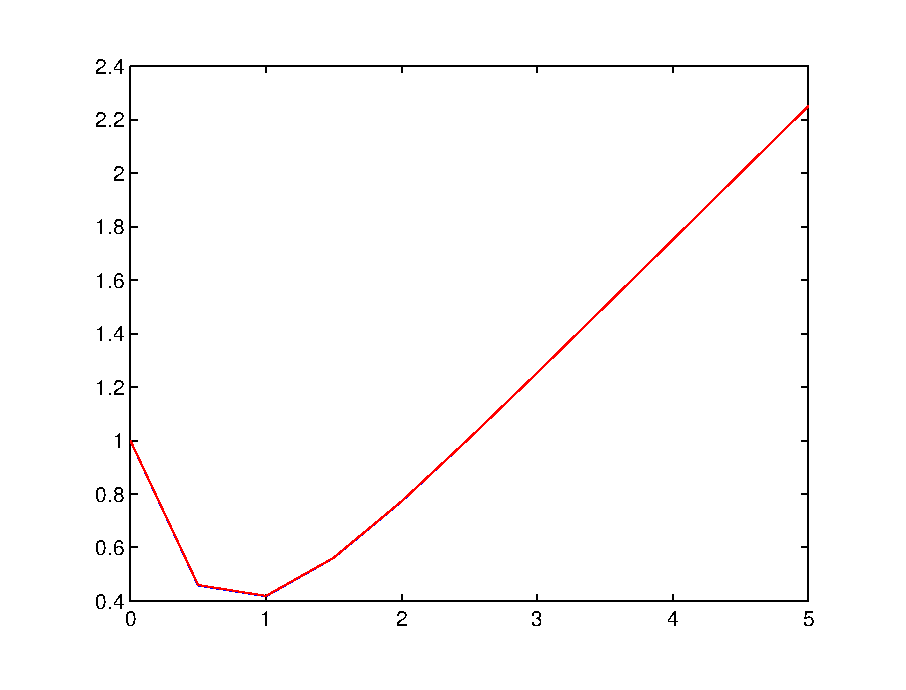
\includegraphics[width=0.6\textwidth]{Taylor}\\
\caption{泰勒级数法}
\end{figure}

\section{龙格库塔法}
\subsection{基本思想}
泰勒公式表面上看形式简单,但具体构造时往往很困难,因为按迭代式求导,这一过程可能很复杂。
因此通常不直接用泰勒公式,而借鉴其思想提出其它公式。\\
龙格库塔法的基本思想:\par
若在$[x_k, x_{k+1}]$上多预测几个点的斜率值,然后将它们的算术平均作为平均斜率,则有可能构造出具有更高精度的计算公式。
\subsection{二阶龙格库塔法}
将改进欧拉法推广为:
\begin{equation}
\left\{ \begin{array}{l}
y_{k + 1}=y_k + h[\lambda_1 K_1+\lambda_2 K_2]\\
K_1=f(x_k,y_k)\\
K_2= y_k + f(x_k + ph, y_k +phK_1)]
\end{array} \right.
\end{equation}
首先希望能确定系数 $K_1$、$K_2$、$p$,使得到的算法格式有2阶精度,即在${y_k} = y(x_k)$的前提假设下,使得
\[{R_k} = y({x_{k + 1}}) - {y_{k + 1}} = O({h^3})\]
步骤一: 将$K_2$在 $(x_k,y_k)$ 点作泰勒展开:
\[\begin{array}{l}
K_2= f({x_k} + ph\;,\,\;{y_k} + ph{K_1})\\
\ \ \quad= f({x_k}\,,\,\;{y_k}) + ph{f_x}({x_k}\,,\,\;{y_k}) + ph{K_1}{f_y}({x_k}\,,\,\;{y_k}) + O({h^2})\\
\ \ \quad= y'({x_k}) + phy''({x_k}) + O({h^2})
\end{array}\]
步骤二: 将 $K_2$ 代入式(5.2.1)的第一个式子,得到
\[\begin{array}{l}
{y_{k + 1}} = {y_k} + h\,\left\{ {\;{\lambda _1}\;y'({x_k}) + {\lambda _2}\;[y'({x_k}) + phy''({x_k}) + O({h^2})]\;} \right\}\\
\ \ \ \ \ \ = {y_k} + ({\lambda _1}\, + {\lambda _2})h\,y'({x_k}) + {\lambda _2}\,p{h^2}y''({x_k}) + O({h^3})
\end{array}\]
步骤三: 将 $y_{k+1}$与 $y(x_{k+1})$ 在 $x_k$ 点的泰勒展开作比较
\[{y_{k + 1}} = {y_k} + ({\lambda _1}\, + {\lambda _2})h\,y'({x_k}) + {\lambda _2}\,p{h^2}y''({x_k}) + O({h^3})\]
\[y({x_{k + 1}}) = y({x_k}) + hy'({x_k}) + \frac{{{h^2}}}{2}y''({x_k}) + O({h^3})\]
要求${R_k} = y({x_{k+ 1}}) - {y_{k + 1}} = O({h^3})$,则必须有:
\[{\lambda _1} + {\lambda _2} = 1\;,\;\;\;{\lambda _2}p = \frac{1}{2}\]
存在无穷多个解。所有满足上式的格式统称为2阶龙格库塔格式。
注意到,$p = 1,\;\;{\lambda _1} = {\lambda _2} = \frac{1}{2}$就是梯形法。\par
二阶龙格库塔公式用多算一次函数值f的办法避开了二阶泰勒级数法所要计算的f 的导数。在这种意义上,可以说龙格库塔方法实质上是泰勒级数法的变形。

\subsection{经典四阶龙格库塔法}
高阶龙格库塔法的构造和二阶类似,下面给出经典的四阶龙格库塔法:
\[\left\{ {\begin{array}{*{20}{l}}
{{y_{k + 1}} = {y_k} + \frac{h}{6}({K_1} + 2{K_2} + 2{K_3} + {K_4})}\\
{{K_1} = f({x_k},{y_k})\quad \quad \quad \quad \quad \quad \quad \quad \;\;}\\
{{K_2} = f({x_k} + \frac{h}{2},{y_k} + \frac{h}{2}{K_1})\quad \quad \quad \quad }\\
{{K_3} = f({x_k} + \frac{h}{2},{y_k} + \frac{h}{2}{K_2})\quad \quad \quad \quad }\\
{{K_4} = f({x_k} + h,{y_k} + h{K_3})\quad \quad \quad \quad \quad }
\end{array}} \right.\]

\subsection{龙格库塔法的Matlab实现}
以下是部分的龙格库塔法的Matlab代码\footnote{此代码由王嘉乐提供}局部:

\begin{quote}
\small{    c = subs(f,[x,y],[j(i,1),j(i,2)]);\\
    d = subs(f,[x,y],[j(i,1)+h/2,j(i,2)+h*c/2]);\\
    e = subs(f,[x,y],[j(i,1)+h/2,j(i,2)+h*d/2]);\\
    g = subs(f,[x,y],[j(i,1)+h,j(i,2)+h*e]);\\
    j(i+1,2) = j(i,2) + (c+2*d+2*e+g)*h/6;\\
    j(i+1,1) = j(i,1) + h;\\
    k(i+1,2) = k(i,2) + subs(f,[x,y],[k(i,1),k(i,2)])*h;\\
    k(i+1,1) = k(i,1) + h;           \% Eular-method\\
    l(i+1,1) = l(i,1)+ h;\\
    l(i+1,2) = exp(1-cos(l(i+1,1)));\% 原函数
}
\end{quote}
Figure 5给出了代码的输出结果,显示四阶龙格库塔法和精确解几乎完全相等。\par
\begin{figure}
  \centering
  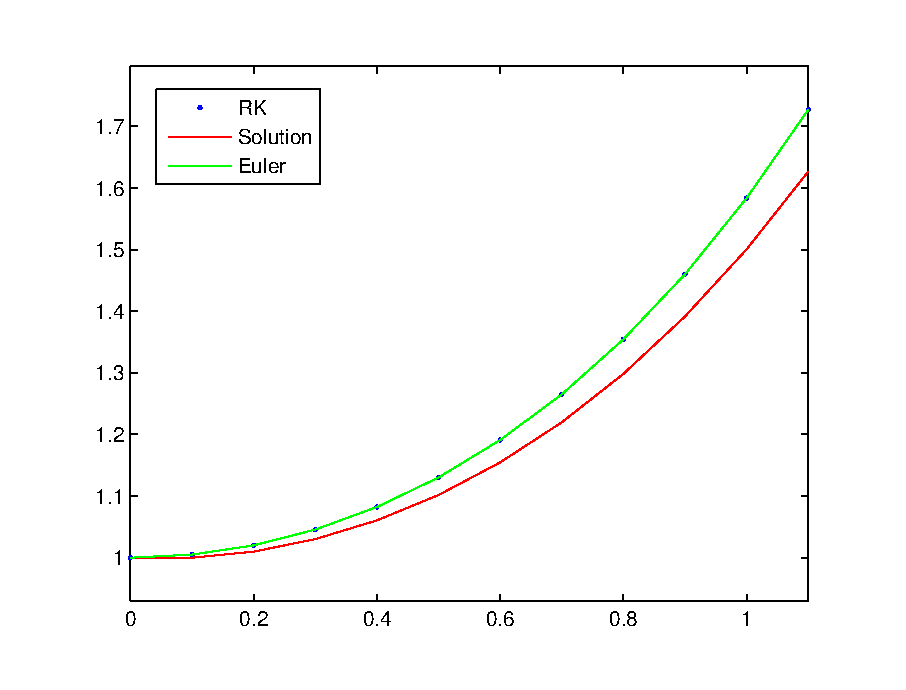
\includegraphics[width=0.65\textwidth]{RK}\\
  \caption{四阶龙格库塔法}
\end{figure}
下表给出了具体的比较数据:
\begin{center}
    \begin{tabular}{|l|l|l|l|l|}
  \hline
x&Solution&Euler&RK&Error RK\\
\hline
0&1&1&1&0\\
0.1&1.005008335&1&1.005008335&1.46228E-10\\
0.2&1.02013342&1.009983342&1.020133419&4.21571E-10\\
0.3&1.045675943&1.030048613&1.045675942&5.72453E-10\\
0.4&1.082138316&1.060488631&1.082138316&1.76393E-10\\
0.5&1.130225801&1.101786004&1.130225803&-1.5678E-09\\
0.6&1.190846478&1.154608438&1.190846484&-6.10025E-09\\
0.7&1.265108387&1.219802535&1.265108403&-1.5776E-08\\
0.8&1.354311579&1.298384372&1.354311613&-3.411E-08\\
0.9&1.459932186&1.391524765&1.459932252&-6.59338E-08\\
1&1.583595065&1.500526645&1.583595183&-1.17397E-07\\
1.1&1.727031028&1.626791608&1.727031223&-1.95752E-07\\
\hline
\end{tabular}
\end{center}

\section{亚当姆斯法}
\subsection{基本描述}
一般地,利用插值原理所建立的一系列数值积分方法也可以导出解微分方程的一系列计算公式。
运用插值方法的关键在于选取合适的插值节点。假设已构造出$f(x,y(x))$的插值多项式$P_r(x)$,则
\[\begin{array}{l}
\int_{{\kern 1pt} {x_n}}^{{\kern 1pt} {x_{n + 1}}} {f(x,y(x))dx}  \approx \int_{{\kern 1pt} {x_n}}^{{\kern 1pt} {x_{n + 1}}} {{P_r}(x)dx} \\
 \Rightarrow {y_{n + 1}} = {y_n} + \int_{{\kern 1pt} {x_n}}^{{\kern 1pt} {x_{n + 1}}} {{P_r}(x)dx}
\end{array}\]
利用$r+1$个节点上的被积函数值构造$r$阶牛顿后插多项式, 有
\[{N_r}({x_n} + t{\kern 1pt} h)\; = \sum\limits_{j = 0}^r {{{\left( { - 1} \right)}^j}} \left( {\begin{array}{*{20}{c}}
{ - t}\\
j
\end{array}} \right){\Delta ^j}{f_{n - j}}\]
其中,$0 \le t = \frac{{x - {x_n}}}{h} \le 1$,${\Delta ^j}$表示$j$阶向前差分。
\[\int_{{\kern 1pt} {x_n}}^{{\kern 1pt} {x_{n + 1}}} {f(x,y(x))\,dx\mathop  = \limits^{x = {x_n} + th} \int_{{\kern 1pt} 0}^{{\kern 1pt} 1} {{N_r}({x_n} + t{\kern 1pt} h)\,h\,dt + } } \int_{{\kern 1pt} 0}^{{\kern 1pt} 1} {{R_r}({x_n} + t{\kern 1pt} h)\,h\,dt} \]
于是有,
\[\begin{array}{l}
{y_{n + 1}} = {y_n} + h\int_{{\kern 1pt} 0}^{{\kern 1pt} 1} {{N_r}(} {x_n} + t{\kern 1pt} h)\,dt = {y_n} + h\sum\limits_{j = 0}^r {\int_{{\kern 1pt} 0}^{{\kern 1pt} 1} {{{\left( { - 1} \right)}^j}\left( {\begin{array}{*{20}{c}}
{ - t}\\
j
\end{array}} \right)} {\Delta ^j}{f_{n - j}}dt} \\
 = {y_n} + h\sum\limits_{j = 0}^r {\int_{{\kern 1pt} 0}^{{\kern 1pt} 1} {{{\left( { - 1} \right)}^j}\left( {\begin{array}{*{20}{c}}
{ - t}\\
j
\end{array}} \right)} dt} {\Delta ^j}{f_{n - j}} = {y_n} + h\sum\limits_{j = 0}^r {{\alpha _j}} {\Delta ^j}{f_{n - j}}
\end{array}\]
其中${\alpha _j} = \int_{{\kern 1pt} 0}^{{\kern 1pt} 1} {{{\left( { - 1} \right)}^j}\left( {\begin{array}{*{20}{c}}
{ - t}\\
j
\end{array}} \right)} dt$
实际计算时,将差分展开
\[
{\Delta ^j}{f_{n - j}}\; = \sum\limits_{i = 0}^j {{{\left( { - 1} \right)}^i}} \left( {\begin{array}{*{20}{c}}
j\\
i
\end{array}} \right){f_{n - i}}\]
\[\sum\limits_{j = 0}^r {{\alpha _j}} {\Delta ^j}{f_{n - j}} = \sum\limits_{j = 0}^r {{\alpha _j}} \sum\limits_{i = 0}^j {{{\left( { - 1} \right)}^i}} \left( {\begin{array}{*{20}{c}}
j\\
i
\end{array}} \right){f_{n - i}} = \sum\limits_{i = 0}^r {\left[ {{{\left( { - 1} \right)}^i}\sum\limits_{j = i}^r {\left( {\begin{array}{*{20}{c}}
j\\
i
\end{array}} \right){\alpha _j}} } \right]} {f_{n - i}} = \sum\limits_{i = 0}^r {{\beta _{ri}}} {f_{n - i}}
\]
\[ \Rightarrow {y_{n + 1}} = {y_n} + h\sum\limits_{i = 0}^r {{\beta _{ri}}} {f_{n - i}}\]
局部截断误差为:
\[\begin{array}{l}
{R_r} = y({x_{n + 1}}) - {y_{n + 1}} = h\int_{{\kern 1pt} 0}^{{\kern 1pt} 1} {{R_r}({x_n} + t{\kern 1pt} h)\,dt} \\
 = h\int_{{\kern 1pt} 0}^{{\kern 1pt} 1} {\frac{{{y^{(r + 2)}}\left( {{\xi _n}} \right)}}{{\left( {r + 1} \right)!}}{\omega _{r + 1}}\left( t \right)dt}  = {B_r}{h^{r + 2}}{y^{(r + 2)}}({\xi _n})\\
 \approx {B_r}{h^{r + 2}}{y^{(r + 2)}}({x_n})
\end{array}\]
常用的$r=3$的四阶公式:
\begin{equation}
{y_{i + 1}} = {y_i} + \frac{h}{{24}}(55{f_i} - 59{f_{i - 1}} + 37{f_{i - 2}} - 9{f_{i - 3}})
\end{equation}
\[R \approx \frac{{251}}{{720}}{h^5}{y^{(5)}}({x_n})\]

\subsection{Matlab代码实现}
以下是亚当姆斯法的Matlab代码\footnote{此代码有骆韬提供}部分:
\begin{quote}
\small{
p =  y(4) + h/24*difl*[-9 37 -59 55]'; \%predictor\\
x(5) = x(4) + h\\
difl(5) = func(x(5),p);\\
y(5) = y(4) + h/24*[1 -5 19 9]*difl(2:5)';\\
hi = x(5)\\
hello = y(5)\\
}
\end{quote}
代码编译出来的结果见Figure 6:
\begin{figure}
  \centering
  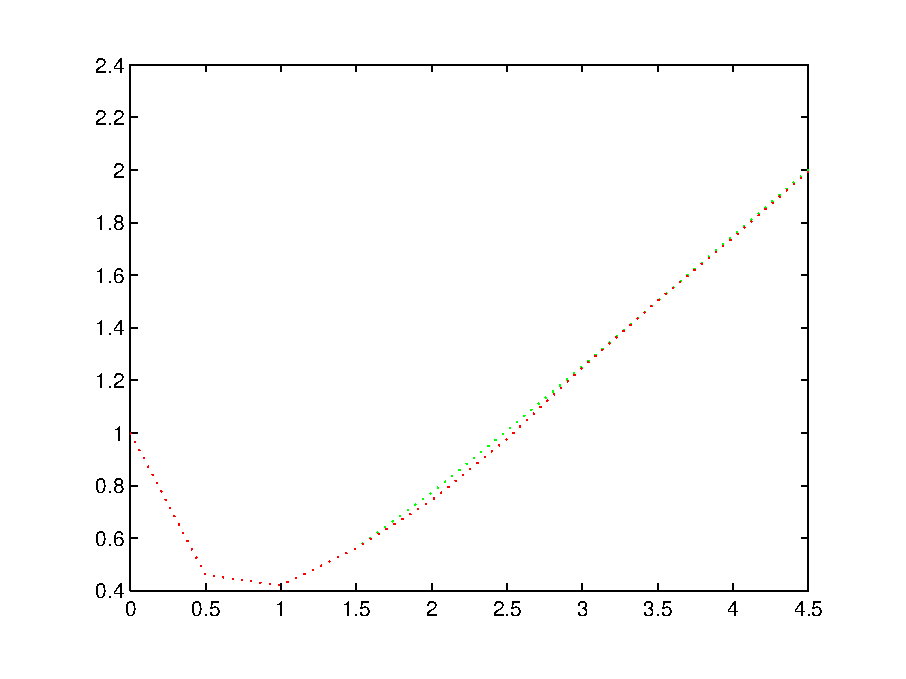
\includegraphics[width=0.65\textwidth]{Adams}\\
  \caption{亚当姆斯法}
\end{figure}

\begin{center}
    \begin{tabular}{|l|l|l|}
       \hline
x&exact solution&adams\\
\hline
0&1&1\\
0.5&0.459849302&0.459849302\\
1&0.419169104&0.419169104\\
1.5&0.562233836&0.562233836\\
2&0.772894549&0.743309432\\
2.5&1.008422434&0.977044821\\
3&1.25309844&1.248469209\\
3.5&1.501139852&1.502978241\\
4&1.750419328&1.741781699\\
4.5&2.000154262&1.994588882\\
       \hline
     \end{tabular}
\end{center}




\section{一种新的变步长的欧拉法--ZWL法}
\subsection{方法的产生和基本算法}
在普通的欧拉法中,我们将区间$[a,b]$ $n$等分,步长固定为$h=(b-a)/n$。对于这类补偿恒定的数值方法,显然当步长越小时,
其精度就会越高,但是另一方面又会引入计算量翻倍的问题。对于计算机而言,计算量很大程度上决定其运算效率,所以,如果我们
在相同的计算量的前提上,如果能够得到一个更加精确的数值解,将是非常乐观的。\par
之所以有变步长的想法,这是因为对一般的初值问题,解的图像在某些区域的误差随着步长的减小并没有得到较大幅度的降低,而另一些
区域可能这种变化就会比较大。所以,我们就可以选择性的改变某些区域的步长。直观的感觉告诉我们,当曲线和直线的相似度高(实际上
简单的想法是:在$y(x)$图像中,$y'(x)$的值越大说明斜率越大,所以补偿应该定的短一些。反之,$y'(x)$(绝对值)小时,我们定出来的步长可以适当变大。\par
为了简化代码以及运算的复杂度,我们就先没有直接利用曲率。但是在趋势上,步长和
$|y'(x)|$是一种反相关的关系。为此,我们开始的模型是简单的反比关系,但是很快就会有麻烦。首先是当$|y'(x)|$
很小时,部分区域就会有十分夸张的大的步长,总而使得作用失效;另一方面,$|y'(x)|$如果很大并且其“调和级数”是收敛的话,就会出
现不能得到x比较大的对应的y的数值解。为此,综合上述所有的因素,我们引入了两个参量,得到下式
\begin{equation}
h_k=\frac{A}{\left|f(x_k,y_k)\right|+B}+C
\end{equation}
其中$A,B,C$为待定参数。

于是我们得到求解问题的ZWL初步方法:
\begin{equation}
\left\{ \begin{array}{l}
{y_{k + 1}} = {y_k} + \left(\frac{A}{\left|f(x_k,y_k)\right|+B}+C\right)f({x_k},{y_k}),\quad i = 1,2, \cdots ,n - 1\\
{y_0} = y({x_0})
\end{array} \right.
\end{equation}



\subsection{ZWL初步方法的定性判断}
前文中我们一直很强调计算量的问题,所以在考察该ZWL法与普通欧拉法,梯形法等的算法优越与否时,我们应该有一个合理的比较方式。
为此,正对这一情况,我们首先选定一个特定的区间$[x_0,x_n]$然后根据欧拉法我们可以得到$n$段相等的步长,可以很简单的写出代码。对于我们
的变步长的方法,我们将调节$A,B,C$三个参数,使得在区间$[x_0,x_n]$同样也有$n$段步长(步数相等),但是显然每段步长不等,然后代入上述的
迭代公式$(5.0.2)$。\par
ZWL法和泰勒级数法不好直接比较。但是可以看到的是n阶的泰勒级数法的运算量不仅和步数有关,还和阶数有关,因为我们要在代码中体现
阶数的运算。因此,如果要进一步的比较的话,就需要计算泰勒级数法的运算量,因此ZWL法就会有
更多的步数。但是两者的具体误差比较取决于具体的函数和泰勒法的阶数。

\subsection{ZWL初步方法和欧拉法的Matlab示例对比}
为了更好的了解ZWL的初步方法,我们通过求解如下初值问题来描述$ZWL$法和欧拉法的误差能力:
\begin{equation}
    \left\{
      \begin{array}{ll}
        y'(x)=y\sin{x} \\
        y(0)=1
      \end{array}
    \right.
\end{equation}

以下是我们的Matlab代码\footnote{此代码由骆韬提供}局部\footnote{省去简单的变量和参量的初始化},两种方法的步数都为10,我们估计$y(5)$:
\begin{quote}
\small{
c = [x0,y0,x0,y0];\\
for i = 2:n\\
    h = abs(5/(subs(f,[x,y],[c(i-1,1),c(i-1,2)])+10)+0.01);\%ZWL法的步长\\
    c(i,2) = c(i-1,2) + subs(f,[x,y],[c(i-1,1),c(i-1,2)])*h;\\
    c(i,1) = c(i-1,1) + h;\\
end\\
for i = 2:n\\
    c(i,4) = c(i-1,4) + subs(f,[x,y],[c(i-1,3),c(i-1,4)])*h;\\
    c(i,3) = c(i-1,3) + h;\%此处的h是初始的h=0.5\\
end\\
plot(c(:,1),c(:,2))\%ZWL法\\
hold on\\
plot(0:0.1:5,subs(ff,0:0.1:5))\%方程的解\\
hold on\\
plot(c(:,3),c(:,4))\%欧拉法\
}
\end{quote}

运行上述代码后得到图像Figure 7:
\begin{figure}[htpb]
\centering
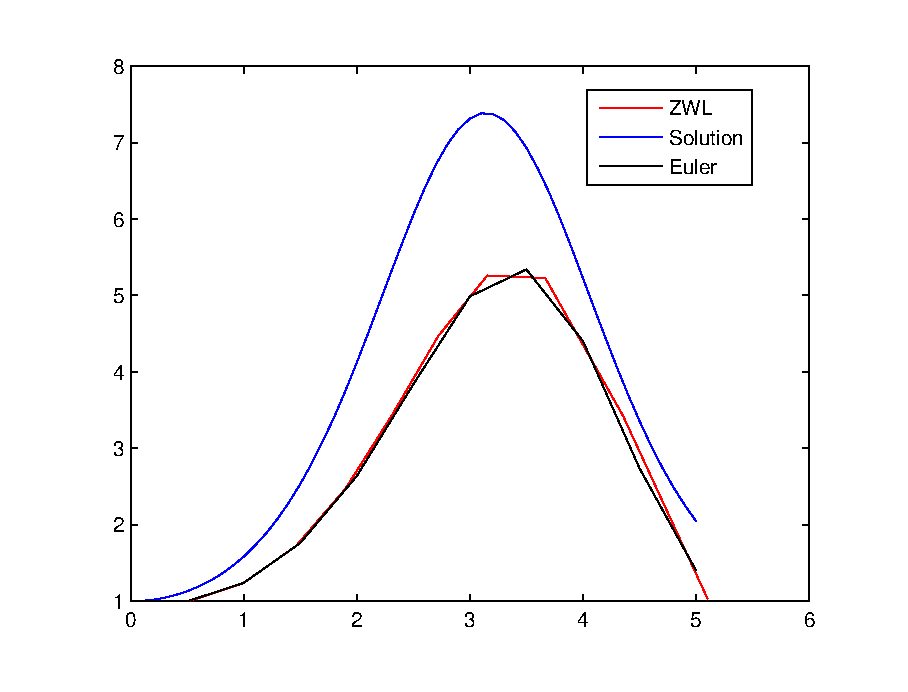
\includegraphics[width=0.65\textwidth]{Euler_ZWL}
\caption{欧拉法和ZWL初步法的对比}
\end{figure}
\par
从上图已经可以很容易的看出,很不幸的是,欧拉法和ZWL法的误差是不相上下的,更多的实例表明ZWL的变步长并不会使误差比欧拉法的误差更高阶。

一个比较简单的证明的思路是这样的:考虑到$B\ C$两个参数实质上只是为了防止计算时的溢出,所以在讨论误差和精度时可以忽略。而忽略它们以后就会发现:$\left(\frac{A}{\left|f(x_k,y_k)\right|+B}+C\right)f({x_k},{y_k})$就变成了
$\left(\frac{A}{f(x_k,y_k)|}\right)f({x_k},{y_k})=|A|$,这就看出来相当于是调换了一下$x,y$的地位,把$y$看成自变量以后,$y$就是等步长的欧拉法。所以说,这种方法的实质其实是几乎没有多大的作用
的。同时这也说明了一个趋势,我们的数值方法基本都是基于欧拉法发展的,变步长的方法没有得到很好地发展\footnote{可以作为辅助算法}也是有原因的,而另两个方向:高阶和多步得到了很好地
改进。

\subsection{ZWL法}
当然,我们也没有完全放弃变步长,进一步的我们知道平面曲线的曲率的计算式如下:
\[\rho=\frac{|y''|}{\left(\sqrt{1+y'^2}\right)^3}\]
同样如果我们将式5.1.1中的$|f(x_k,y_k)|$换成$\rho_k$的话,也可以引入$B\ C$两个参量,从而可以简化上式,将1去掉。
于是我们有:
\begin{equation}
h_k=\frac{A}{\frac{|y''(x_k)|}{f(x_k,y_k)^3}+B}+C
\end{equation}
由此得到ZWL法(将$h_k$代入欧拉法的公式即可)

同样我们也比较一下它和欧拉法的"优劣"。
我们研究如下的初始问题:
\begin{equation}
    \left\{
      \begin{array}{ll}
        y'(x)=x-2 y\\
        y(0)=1
      \end{array}
    \right.
\end{equation}

以下是我们的Matlab代码\footnote{此代码由张文超提供}局部,两种方法的步数都为10,我们估计$y(5)$:
\begin{quote}
\small{
fx = diff(f,x) + diff(f,y)*f;\\
fe = 0.25*(-1+5*exp(-2*x)+2*x);\\
n=11;\\
c=[x0,y0,x0,y0,x0,y0];\\
for i=2:n\\
    A=subs(fx,[x,y],[c(i-1,5),c(i-1,6)])/((subs(f,[x,y],[c(i-1,1),c(i-1,2)])$\wedge$3)+20);\\
    h1 = abs(0.03164*(1/A)+0.05);\\
    c(i,2) = c(i-1,2) + subs(f,[x,y],[c(i-1,1),c(i-1,2)])*h1;\\
    c(i,6) = c(i-1,6) + subs(f,[x,y],[c(i-1,5),c(i-1,6)])*h1;\\
    c(i,1) = c(i-1,1) + h1;\\
}
\end{quote}

运行上述代码后得到图像Figure 8\&9并且有下列表格:
\begin{figure*}
\begin{minipage}[t]{0.5\textwidth}
\centering
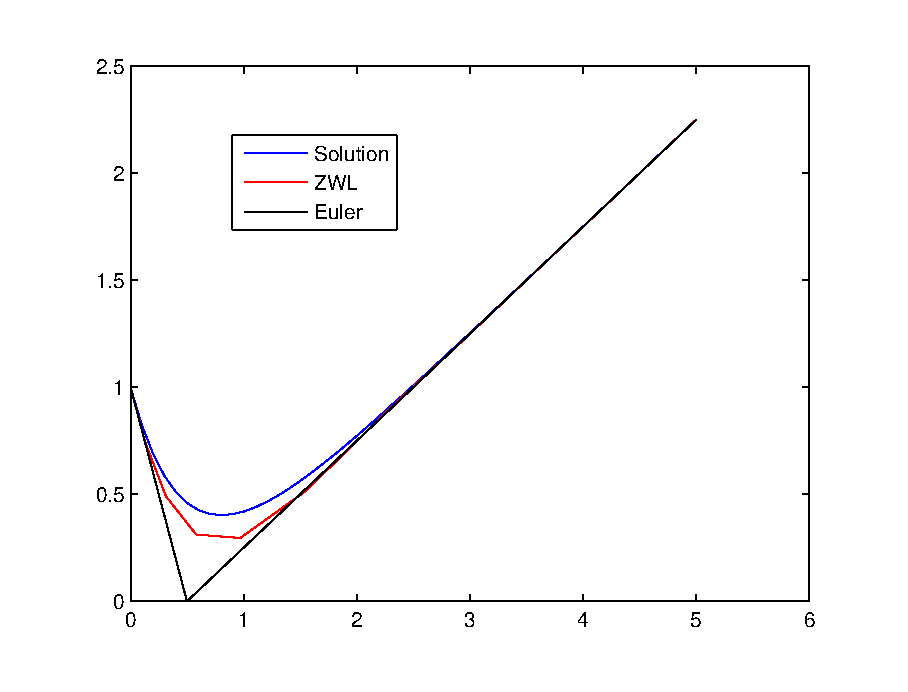
\includegraphics[width=\textwidth]{ZWL}
\caption{ZWL法和欧拉法比较图}
\end{minipage}%
\begin{minipage}[t]{0.5\textwidth}
\centering
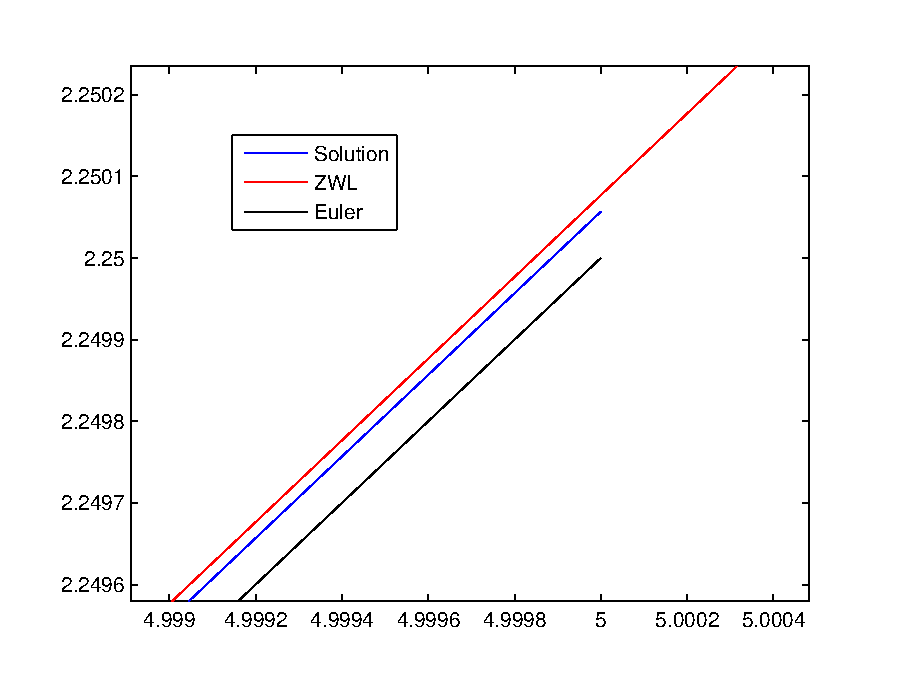
\includegraphics[width=\textwidth]{ZWL_B}
\caption{ZWL法和欧拉法比较放大图}
\end{minipage}%
\end{figure*}

\begin{center}
\begin{tabular}{|l|l|l|l|}
  \hline
x&欧拉法误差&x&ZWL误差\\
\hline
0&0&0&0\\
0.5&0.459849301&0.125936&0.03652029\\
1&0.169169104&0.314040874&0.083674342\\
1.5&0.062233835&0.581511957&0.119386018\\
2&0.022894549&0.970246307&0.119171276\\
2.5&0.008422434&1.552038295&0.065958008\\
3&0.00309844&2.260075996&0.009500218\\
3.5&0.001139852&2.938377772&0.004970116\\
4&0.000419328&3.628202798&0.000325756\\
4.5&0.000154262&4.313800002&0.000230361\\
5&5.67499E-05&5.000985849&2.06671E-05\\
  \hline
\end{tabular}
\end{center}

\par
我们可以看到改进后的ZWL法还是比欧拉法更有效的,这是因为真正起到作用步长的部分存在二阶导数,所以它的误差相应的就不再是一阶无穷小量了。
当然,ZWL对于一些曲率变化比较悬殊的函数效果会更好。从总的方面来说,ZWL法还是优于欧拉法的。

\subsection{ZWL法的收敛性简单证明}
\begin{proof}
    因为\[y_{k+1}=y_k+h_kf(x_k,y_k)=y_{k}+\left(\frac{A}{\frac{|y''(x_k)|}{f(x_k,y_k)^3}+B}+C\right)f(x_k,y_k)\]
而由于$A,B,C>0$,故$h_k$满足不等式$C<h_k\leq \frac{A}{B}+C$
在实际参数选择的过程中,只要令$\frac{A}{B}+C<1$就可以使得
$|y_{k+1}-y_{k}|\leq L^{k}|y_1-y_0|$
其中$0<L<1$,故$$\lim_{k\rightarrow\infty}|y_{k+1}-y_{k}|=0$$
所以ZWL法收敛。
\end{proof}


\section{组员的任务分配}
张文超:负责撰写文章(统稿);并对ZWL方法做了一定的理论分析;提供了ZWL法的最终代码\par
王嘉乐:负责编写程序比较各个数值方法的优越性(提供了simposon的idea);给出了四阶龙格库塔法的代码以及文中的绝大多数表格\par
骆韬:负责编写泰勒法代码以及比较ZWL方法与普通欧拉法方法的区别,给出了亚当姆斯法的代码\par
ZWL法是由张文超先提出的根据曲线变化改变步长的想法,由王嘉乐、骆韬共同得到比较简单的ZWL初步方法。在试验的过程中又发现了一些问题:
开始认为ZWL已经比欧拉法好了,但是发现存在示例和此结论有冲突。后期由张文超继续完善曲率的ZWL法。\par
后期的Project要求的三道题目由骆韬和王嘉乐完成,其中骆韬提供了Airy方程的求解代码。\par


\section{附录:project要求的几道实例}
\subsection{a)}
前面已经给出了一般的Taylor级数的Matlab代码,故不重述。以下Figure10和Figure11
是 a1 \& a2的数值结果:
\begin{figure*}
\begin{minipage}[t]{0.5\textwidth}
\centering
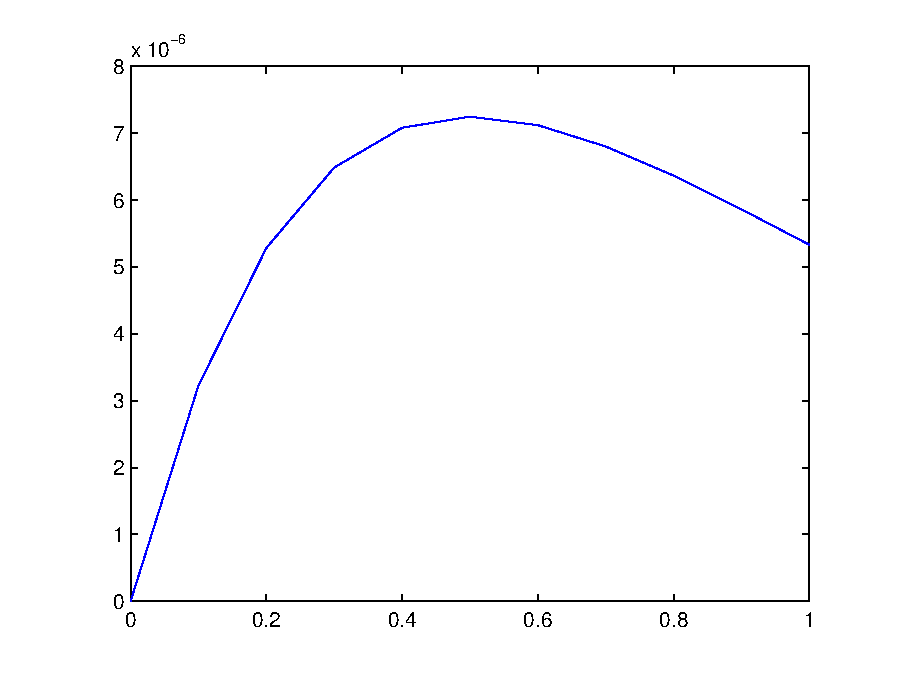
\includegraphics[width=\textwidth]{a1}
\caption{a(i)的数值解图}
\end{minipage}%
\begin{minipage}[t]{0.5\textwidth}
\centering
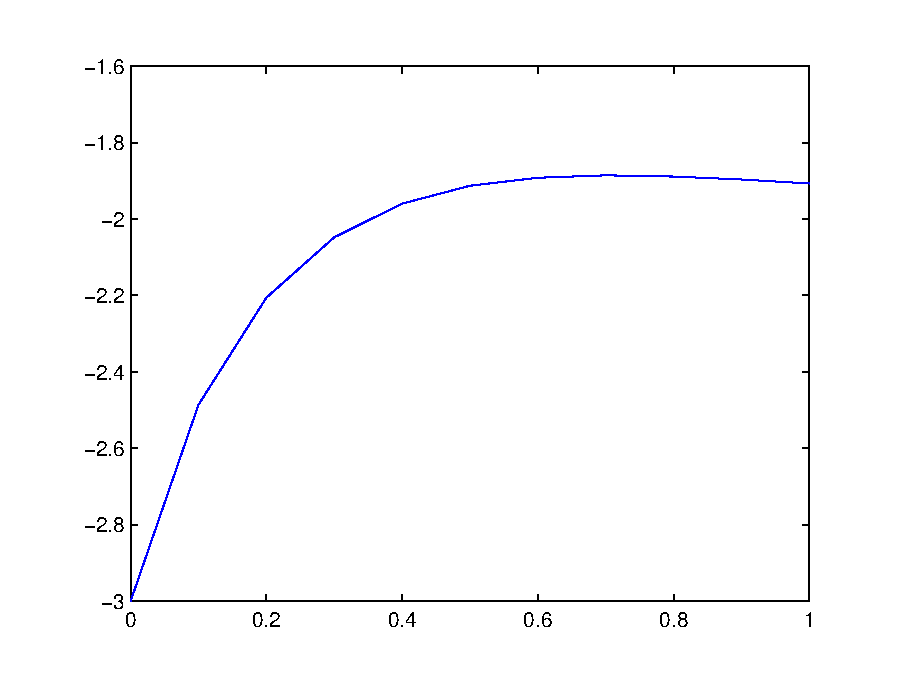
\includegraphics[width=\textwidth]{a2}
\caption{a(ii)的数值解图}
\end{minipage}%
\end{figure*}

\par
所以我们得到的$y(1)$分别为:0.4191744355和0.2384054319。
\subsection{b)}
先给出此题的源代码主要部分\footnote{王嘉乐提供}:
\begin{quote}
\small{
c(i) = diff(c(i-1),x) + diff(c(i-1),y)*c(1); \%各阶导数\\
subs-c = subs(c,[x,y],[x0,y0]);\\
taylor = taylor + (subs-c(i)*(x-x0)$\wedge$ i)/factorial(i);  \%n阶taylor展开\\
 b(i) = subs(taylor,[x0,y0,x],[a(i-1),b(i-1),a(i)]);\\
 k(i,2) = k(i-1,2) + subs(f,[x,y],[k(i-1,1),k(i-1,2)])*h;\\
    k(i,1) = k(i-1,1) + h;\\
    k(i,2) = k(i-1,2) + subs(f,[x,y],[k(i-1,1),k(i-1,2)])*h;\\
    k(i,1) = k(i-1,1) + h;\\
}
\end{quote}
由上述的代码输出的结果见下表:\\
\begin{center}
\begin{tabular}{|l|l|l|}
  \hline
  % after \\: \hline or \cline{col1-col2} \cline{col3-col4} ...
  方法 & $\phi(1)$的估计 & $\phi(3)$的估计 \\
  \hline
  步长0.1欧拉法 & 0.9153 & -0.9707 \\
  步长0.01欧拉法 & 0.9089 & -0.9432 \\
  二阶泰勒法 & 1.0000 & -1.0800 \\
  五阶泰勒法 & 0.9083 & -0.9410  \\
  \hline
  精确到千分之一的精确值 & 0.9082 & -0.9402 \\
  \hline
\end{tabular}
\end{center}

\par
显然五阶泰勒法得到的估计最准确,拥有五阶无穷小的截断误差。用五阶泰勒法可以得到$\phi(10)=-0.9109$。

\subsection{c)}
艾里方程是以英国英格兰天文学家、数学家乔治·比德尔·艾里命名的二阶线性微分方程,他在1838年研究光学的时候遇到了这个函数。
Ai(x)(艾里函数)与相关函数Bi(x)(也称为艾里函数),是艾里方程的解:
\begin{equation}\label{Airy Equation}
    y''(x)=xy
\end{equation}
艾里函数有个特点,它有一个转折点,在这一点函数由周期性的振动转变为指数增长(或衰减)。
下面是Ariy方程的泰勒法数值解的Matlab代码\footnote{代码由骆韬提供}局部,Figure 12为输出解的图像:
\begin{quote}
\small{
syms x y x0 y0 y1; \% 一阶导数是y1;y(x0)=y0\\
c = f;\\
for i = 2:5\\
c(i) = diff(c(i-1),x) + diff(c(i-1),y)*c(1); \%\% 各阶导数\\
end\\
subs-c = subs(c,[x,y],[x0,y0]);\\
taylor = y0 +y1*(x-x0);\\
for i= 1:n\\
   taylor = taylor + (subs-c(i)*(x-x0)$\wedge$(i+1))/factorial(i);  \%n阶taylor展开\\
end\\
}
\end{quote}

\begin{figure}
% Requires \usepackage{graphicx}
\centering
  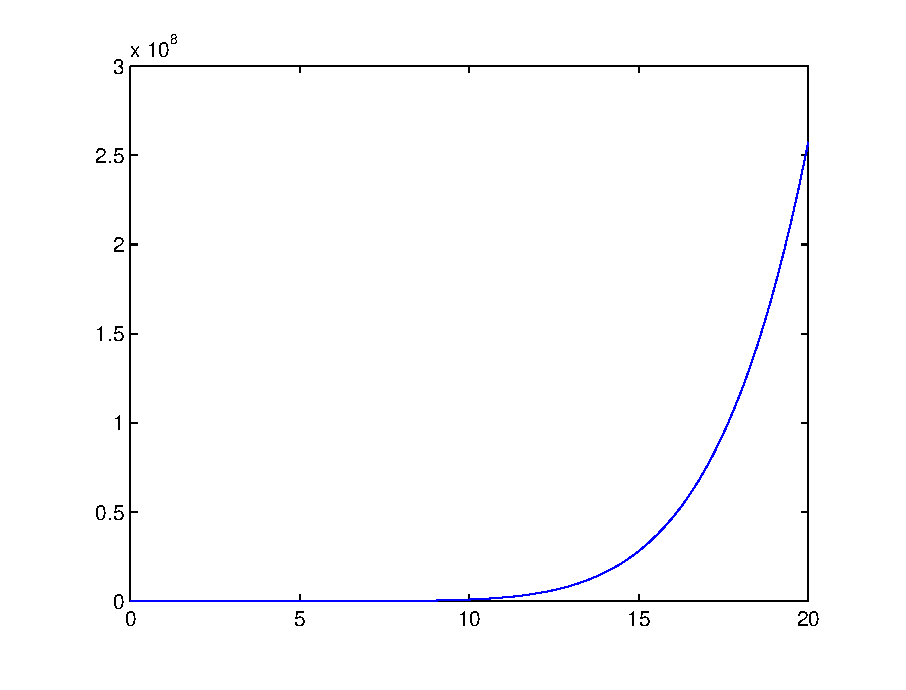
\includegraphics[width=0.65\textwidth]{airy}\\
  \caption{艾里方程的解}
\end{figure}

\newpage

\section{相关程序包}
\begin{itemize}
  \item 欧拉法:eularmethod.m
  \item 泰勒级数法:norderdiff.m
  \item 几种方法比较:Simposonsrule.m
  \item 初步ZWL法:PriZWL.m
  \item ZWL法:ZWL.m
  \item 龙格库塔法:RK.m
  \item 亚当姆斯法:abm.m;func.m;main.m
  \item 例题1:a.m
  \item 例题2:b.m
  \item 例题3:Airy.m
\end{itemize}


\renewcommand\refname{参考文献}
\begin{thebibliography}{99}
\bibitem{lip} 蒋健飞,胡良剑,唐俭.数值分析及\textbf{Matlab}实验[M].科学出版社,2002:274-305.            %参考文献内容
\bibitem{converge} 袁东锦.计算方法--数值分析[M].南京师范大学出版社,2007:86—90.
\end{thebibliography}
\end{document}
